\documentclass[12pt,a4paper]{report}
\usepackage[a4paper,
    left=1.25in,
    right=1in,
    top=1in,
    bottom=1in]{geometry} % Required for inserting images
\usepackage{fullpage}
\usepackage{mathptmx}
\usepackage{titletoc}
\usepackage[titles]{tocloft}
\usepackage{booktabs}   % For professional table formatting
\usepackage{array}      % For enhanced table control
\usepackage{siunitx}    % For proper number formatting
%\usepackage{geometry}   % To adjust page margins
\usepackage{float}

\usepackage{lipsum}
\usepackage{acronym}
\usepackage{graphicx}
% Add to your main document preamble
\usepackage{tikz}
\usetikzlibrary{shapes,arrows,fit,positioning}
\graphicspath{ {./images/} }
\usepackage{pgfgantt}

% Line spacing
\usepackage{setspace}  
\onehalfspacing  % or use \singlespacing or \doublespacing as needed

% Paragraph spacing
\setlength{\parskip}{0.75em}  % space between paragraphs
\setlength{\parindent}{0pt}   % no indentation (you already have this)

% Custom font sizes for headings
\usepackage{sectsty} % to customize section font sizes

% Normal text font size is already 12pt (from documentclass)

% Normal heading style (like \textbf 12pt) - redefine \normalfont
\renewcommand\normalsize{\fontsize{12}{14}\selectfont} % 12pt font with 14pt baseline skip

% Section headings (14pt)
\sectionfont{\fontsize{14}{16}\selectfont\bfseries} 

% Subsection headings (optional, keep smaller)
\subsectionfont{\fontsize{12}{14}\selectfont\bfseries}

% Chapter (main heading) size (16pt bold centered)
\usepackage{titlesec}
\titleformat{\chapter}[display]
  {\normalfont\bfseries\fontsize{16}{18}\selectfont\centering}
  {\chaptername\ \thechapter}{1em}{}

\renewcommand*\contentsname{Table of Contents}

% Redefine the \numberline command for figures
\newlength{\mylen}
\renewcommand{\cftdotsep}{0.5}
\renewcommand{\cftfigpresnum}{\hspace*{-1.5em}\figurename\enspace}
\renewcommand{\cftfigaftersnum}{:}
\settowidth{\mylen}{\cftfigpresnum\cftfigaftersnum}
\addtolength{\cftfignumwidth}{\mylen}


\renewcommand{\cftdotsep}{0.5}
\renewcommand{\cfttabpresnum}{\hspace*{-1.5em}\tablename\enspace}
\renewcommand{\cfttabaftersnum}{:}
\settowidth{\mylen}{\cfttabpresnum\cfttabaftersnum}
\addtolength{\cfttabnumwidth}{\mylen}


\titlecontents{chapter}
[5.5em] %5.3
{\smallskip}
{\contentslabel[\bfseries{\chaptername}~\thecontentslabel{:}]{5.5em}\textbf}%\thecontentslabel
{\hspace*{-5.5em}\textbf}% unnumbered chapters
{\titlerule*[0.35pc]{.}\contentspage}[\smallskip]%

\titlecontents{section}
[1.5em] % i
{\smallskip}
{\thecontentslabel\enspace}%\thecontentslabel
{\hspace*{-5.5em}}
{\titlerule*[0.35pc]{.}\contentspage}%]

\titlecontents{subsection}
[7.12em] %
{\smallskip}
{\thecontentslabel\enspace}%\thecontentslabel
{\hspace*{7.12em}}
{\titlerule*[0.35pc]{.}\contentspage}

\makeatletter
\renewcommand{\@makechapterhead}[1]{%\vspace*{50 pt}%
{\setlength{\parindent}{0pt}\normalfont
\bfseries\Huge\chaptername{\hspace*{0.25em}}\centering\thechapter{:}\ #1
\par\nobreak\vspace{16 pt}}}
\makeatother

\makeatletter
\renewcommand{\@makeschapterhead}[1]{%\vspace*{50 pt}%
{\setlength{\parindent}{0pt}\normalfont
\bfseries\Huge\centering\ #1
\par\nobreak\vspace{16 pt}}}
\makeatother

\title{Major}
\author{Mahan Sigdel}
\date{May 2025}

\setlength{\parindent}{0pt}

\begin{document}
\begin{titlepage}
    \thispagestyle{empty}
    \begin{center}
    
    \vspace*{\fill} % * makes latex to not ignore the command
    \vspace*{-1cm}
    {\large \textbf{TRIBHUVAN UNIVERSITY
}\par}
{\large \textbf{INSTITUTE OF ENGINEERING
}\par}
\vspace{8pt}
KATHMANDU ENGINEERING COLLEGE

KALIMATI, KATHMANDU
\vspace{24pt}

\begin{figure}[ht]
    \centering
    
\includegraphics[scale=0.45]{images/kec.png}
\end{figure}
\vspace{24pt}
{MAJOR PROJECT PROPOSAL REPORT ON\par}
\vspace{14pt}
{\textbf{ Your Project Title}\par}

\vspace{14pt}
{BY\par}
\vspace{14pt}

{KRITIKA DAHAL - KAT078BEI007\par}
{MAHAN SIGDEL - KAT078BEI009\par}
{NISHANA THAPA - KAT078BEI011\par}
{SABINA GHIMIRE - KAT078BEI016\par}

\vspace{24pt}
{TO\par}
\vspace{14pt}
{DEPARTMENT OF ELECTRONICS, COMMUNICATION AND INFORMATION ENGINEERING\par}
{KATHMANDU, NEPAL\par}
{MAY , 2024\par}

    %\vspace*{\fill}

    \end{center}
\end{titlepage}

\pagenumbering{roman}

\chapter*{Acknowledgement}
\addcontentsline{toc}{chapter}{Acknowledgement}
\label{acknowledgement}
We express our gratitude to our project supervisors, \textbf{Er. Sarina Barahi} and \textbf{Er. Puspha Dhamala} along with our project coordinator\textbf{ Er. Sujan Shrestha} for providing invaluable support and guidance throughout the project. We are deeply thankful to the Department of Electronics, Communication, and Information Engineering at Kathmandu Engineering College for granting us the opportunity to complete our minor project as a part of our syllabus. We wholeheartedly appreciate the esteemed Head of the Department of Electronics, Communication, and Information Engineering, \textbf{Asso. Prof. Er. Suramya Sharma}. We sincerely appreciate the encouragement, support, constructive criticism, and guidance provided by the entire teaching staff at the Department of Electronics, Communication, and Information Engineering.

%\chapter*{Abstract}
%\addcontentsline{toc}{chapter}{Abstract}
%\label{abstract}
%\lipsum[2-4]

\tableofcontents
\thispagestyle{empty}
\addtocounter{page}{-1}
\newpage

\listoffigures
\addcontentsline{toc}{chapter}{List of Figures}
\newpage

\listoftables
\addcontentsline{toc}{chapter}{List of Tables}
\newpage

\chapter*{List of Abbreviation}
\addcontentsline{toc}{chapter}{List of Abbreviation}
\label{abbreviation}
\begin{acronym}
 \acro{MPU}{Motion Processing Unit}
 \acro{IMU}{Inertial Measurement Unit}
 \acro{HCI}{Human-Computer Interaction}
 \acro{DoF}{Degrees of Freedom}
 \acro{VR}{Virtual Reality}
 \acro{AR}{Augmented Reality}
 \acro{PLA}{Polylactic Acid}
 \acro{ESP}{Espressif Systems}
 \acro{IoT}{Internet of Things}
 \acro{I/O}{Input/Output}
 \acro{VAR}{Virtual Augmented Reality}
 \acro{MEMS}{Micro-Electro-Mechanical Systems}
 \acro{DMP}{Digital Motion Processor}
 \acro{TCP/IP}{Transmission Control Protocol/Internet Protocol}
 \acro{CPU}{Central Processing Unit}
 \acro{GPU}{Graphics Processing Unit}
 \acro{Wi-Fi}{Wireless Fidelity}
 \acro{3D}{Three-Dimensional}
 \acro{HZ}{Hertz}
 \acro{RISC}{Reduced Instruction Set Computer}
 \acro{IEEE}{Institute of Electrical and Electronics Engineers}
 \acro{HTTP}{Hypertext Transfer Protocol}
 \acro{IDE}{Integrated Development Environment}
 \acro{API}{Application Programming Interface}
 \acro{EEVEE}{Enhanced Efficient Virtual Environment Engine}
 

\end{acronym}
\newpage

\pagenumbering{arabic}

\chapter{Introduction}
\label{introduction}
\section{Background Theory}
The rapid advancement of human-computer interaction (HCI) technologies has paved the way beyond traditional input devices towards more intuitive interfaces. Among these, Gesture-based systems have emerged as a powerful mode of interaction where users engage with digital systems through physical movements, particularly of the hands. Human hands are capable of complex movements and precise control, making them an ideal medium for gesture-based input. This evolution is particularly significant in applications such as gaming, virtual and augmented reality, assistive technology, and robotics.

Leveraging this, modern wearable systems incorporate a variety of sensors to translate hand and finger gestures into digital commands. The MPU6050, a 6-DoF inertial measurement unit (IMU) combining a 3-axis gyroscope and a 3-axis accelerometer, is widely used for real-time tracking of wrist orientation and movement, crucial for recognizing hand gestures [1], [2]. For detecting finger movements, flex sensors are employed, which vary resistance based on bending, providing analog signals proportional to flexion [3]. Alternatively, mechanical switches, activated by levers attached to finger components, offer a digital input method with tactile feedback. Data from these sensors are processed by microcontrollers like the Arduino Mega, which provides ample I/O support. For seamless interaction with external applications, the ESP8266 Wi-Fi module facilitates wireless data transmission, ensuring low-latency communication between the wearable device and the host system [4].

Device housing commonly utilizes 3D-printed PLA filament, chosen for its lightweight properties, customizability, and suitability for ergonomic wearable enclosures that maintain sensor alignment [5]. In the software domain, gesture data is mapped to real-time responses within a digital environment. Game engines, such as Unreal Engine, support external hardware integration, enabling the visualization of hand movements from a first-person perspective [6]. This establishes a seamless connection between physical actions and virtual reactions, particularly effective in immersive puzzle-based or simulation games. Ultimately, gesture-based input systems enhance user experience by aligning digital control with natural human motion, proving ideal for applications ranging from gaming to assistive technology.

\vspace{1.5\baselineskip} 

\section{Problem Statement}
\vspace{1.5\baselineskip} 

\section{Objectives}
\vspace{1.5\baselineskip} 

\section{Scope}
The project encompasses several key areas for development and future expansion:
\begin{itemize}
    \item Integration with machine learning models to improve gesture recognition accuracy
    \item Addition of haptic feedback for more immersive interaction
    \item Expansion to full-body motion capture using additional wearable sensors
    \item Development of a mobile or desktop interface for visualizing and mapping gestures
    \item Incorporating voice + gesture multimodal control systems
\end{itemize}
\vspace{1.5\baselineskip}
\section{Applications}
The data glove system finds applications in various fields including:
\begin{itemize}
    \item Virtual and Augmented Reality (VAR)
    \item Assistive Technology
    \item Gaming
    \item Robotics Control
    \item Smart Environments / IoT Applications
    \item Educational Tools
\end{itemize}




\chapter{Literature Review}
\label{literaturereview}
\section{Literature Review}

Rautaray, S. S., \& Agrawal, A. (2013) [7], focuses on developing a vision-based gesture recognition system that eliminates the need for physical input devices, allowing users to interact with digital objects using natural hand movements. The system employs computer vision algorithms for gesture detection, segmentation, tracking, and recognition, converting hand gestures into meaningful commands for real-time applications. The study highlights the limitations of traditional input methods, such as keyboards and mice, and emphasizes the advantages of markerless tracking systems in improving usability and immersion in dynamic environments. The proposed system contributes to the growing field of gesture-based interfaces.

Chowdhury and Haque (2013) [8], developed an animatronic hand controller that utilized flex sensors and servo motors, showcasing an innovative approach to robotic hand manipulation. The flex sensors played a crucial role in detecting finger bending motions, translating them into electrical signals that corresponded to hand gestures. These signals were then processed by an Arduino microcontroller, which controlled the servo motors responsible for mimicking natural finger movements. By integrating this sensor-motor system, the researchers enabled precise gesture-based control, allowing for applications in robotic prosthetics, remote-controlled manipulators, and assistive technology. Their work underscored the potential of Arduino-driven systems for creating cost-effective and accessible animatronic solutions, paving the way for further advancements in human-machine interaction and gesture-controlled robotics.

Kumar et al. (2012) [3], introduced the DG5 VHand 2.0, a wireless data glove designed to enhance gesture-based interactions in virtual and augmented reality. The glove featured flex sensors, which captured precise finger movements, and Bluetooth connectivity, ensuring seamless real-time communication with external devices. To process gesture inputs effectively, the researchers employed a K-Nearest Neighbors (K-NN) classifier, allowing their system to recognize complex hand motions with high accuracy. The glove was particularly effective for applications such as air-writing, where users could trace letters mid-air, and 3D sketching, enabling intuitive and immersive design processes within virtual environments. Their findings underscored the potential of wearable sensor technology in expanding the boundaries of human-computer interaction, demonstrating how real-time gesture recognition could improve accessibility, user experience, and creative workflows in emerging technologies.

Sturman and Zeltzer (1994) [9],  conducted an extensive survey of early glove-based input devices, highlighting the technological innovations that laid the foundation for modern hand-tracking systems. Among these, the VPL DataGlove utilized optical fibers to measure finger flexion, providing a level of precision that was groundbreaking at the time. Meanwhile, the Dexterous HandMaster (DHM) relied on Hall-effect sensors, which detected changes in magnetic fields to determine finger movements. These devices represented significant strides in human-computer interaction, offering high-accuracy motion tracking crucial for applications in virtual reality (VR) and robotic control.

Huang (2017) [10], explored the application of the MPU6050 sensor in flight control systems, utilizing its integrated accelerometers and gyroscopes to detect tilt angles with high accuracy. This sensor's ability to measure both linear acceleration and angular velocity made it ideal for stabilizing aircraft movements and ensuring precise orientation tracking.


\chapter{Related Theory}
\label{relatedtheory}
\section{Hardware}
\subsection{FLYSKY Receiver}
The FLYSKY receiver is a compact wireless communication module used in remote-controlled systems to receive control signals from a FLYSKY transmitter. It operates on a 2.4GHz frequency band and supports multiple channels, allowing it to control various actuators such as motors and servos. This receiver is widely used in drones, RC planes, and robots due to its reliable range, low latency, and compatibility with many FLYSKY models. It typically connects directly to a flight controller or electronic speed controller (ESC) for signal routing.
\begin{figure}
\centering
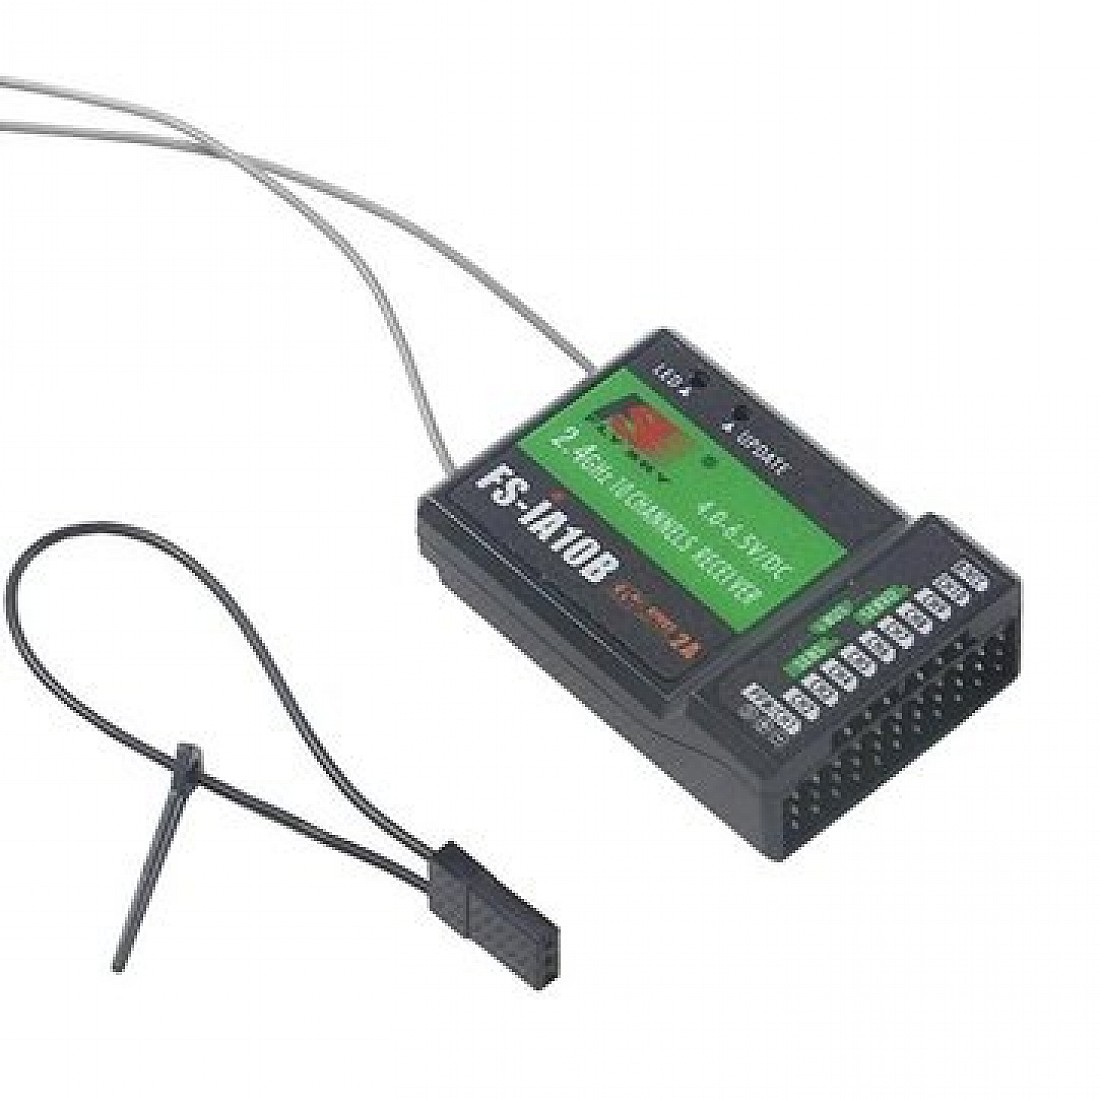
\includegraphics[width=0.5\textwidth]{images/flysky receiver.jpg}
\caption{Raspberry Pi 4 Model B}

\end{figure}

\subsection{30A ESC Skywalker}
The 30A Skywalker ESC (Electronic Speed Controller) is a device designed to control the speed, direction, and braking of a brushless motor. Rated for a maximum continuous current of 30 amps, it is ideal for medium-sized electric drones and RC aircraft. It takes signals from the receiver or flight controller and converts them into three-phase power for the motor, allowing smooth acceleration and precise speed control. The ESC also includes safety features like overheating and overcurrent protection.
\begin{figure}
\centering
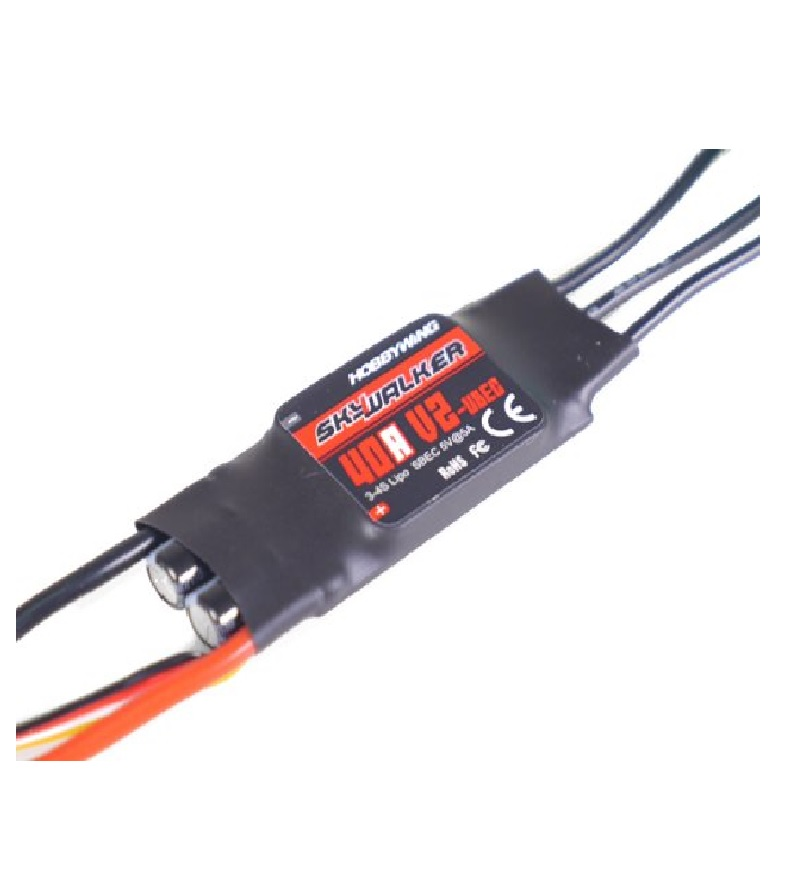
\includegraphics[width=0.5\textwidth]{images/esc.jpg}
\caption{Raspberry Pi 4 Model B}
\end{figure}

\subsection{Flight Stabilizer (NXE4 EVO)}
The NXE4 EVO Flight Stabilizer is an advanced control system used in RC aircraft and drones to maintain stability during flight. It uses onboard sensors such as gyroscopes and accelerometers to detect orientation and movement, and then automatically adjusts control surfaces or motor speeds to correct any deviations. This improves flight performance, especially in windy or unstable conditions, and enables smoother operation for both beginners and experienced pilots. It's essential for autonomous or semi-autonomous flight control.

\subsection{1000KV Brushless Motor}
A 1000KV brushless motor is a high-efficiency electric motor that rotates at 1000 revolutions per minute per volt applied. It is commonly used in drones, RC aircraft, and electric vehicles due to its power-to-weight ratio, reliability, and minimal maintenance needs. Unlike brushed motors, brushless motors have no internal contact between the rotor and stator, reducing wear and increasing lifespan. The motor typically has three wires for connection to an ESC and is paired with a propeller or gear mechanism for motion output.

\subsection{MG996 Metal Gear Servo}
The MG996 is a high-torque, metal gear servo motor used for precise angular movement in robotics, RC vehicles, and automation systems. Its durable metal gear construction offers increased torque and strength compared to plastic gear servos, making it suitable for demanding applications. Controlled by a PWM signal, it can rotate to specific angles between 0° and 180°, making it ideal for steering mechanisms, robotic arms, or flaps in RC aircraft. It comes with a standard 3-wire connector for power, ground, and signal.

\subsection{2200mAh 3S LiPo Battery}
The 2200mAh 3S LiPo (Lithium Polymer) battery is a high-capacity, lightweight power source commonly used in RC models, drones, and portable electronics. With three cells in series, it delivers a nominal voltage of 11.1V and a high discharge rate to support power-hungry components like motors and servos. Its 2200mAh capacity provides moderate runtime, making it ideal for short to medium-duration flights or robotic operations. The battery typically features a discharge plug (like XT60) and a balance connector for safe charging.

\subsection{Buck Module Voltage Regulator}
A buck module voltage regulator is a DC-DC converter that steps down higher input voltage to a lower, stable output voltage. It is commonly used in embedded electronics to power microcontrollers, sensors, and other 5V or 3.3V devices  from higher-voltage sources like LiPo batteries. The module includes components such as an inductor, capacitor, and adjustable potentiometer to maintain a consistent output. Its compact size and efficiency make it essential for battery-powered projects to protect components from over-voltage.

\subsection{Raspberry Pi with USB Camera and HDMI Cable}
The Raspberry Pi is a credit card-sized single-board computer capable of running a full Linux OS and performing various computing tasks. When paired with a USB camera, it can capture images and video for applications like computer vision, surveillance, and robotics. The HDMI cable allows video output to a monitor or display, enabling real-time viewing or debugging. This setup is ideal for lightweight, portable embedded systems where processing power, camera input, and display output are all required.
\begin{figure}
\centering
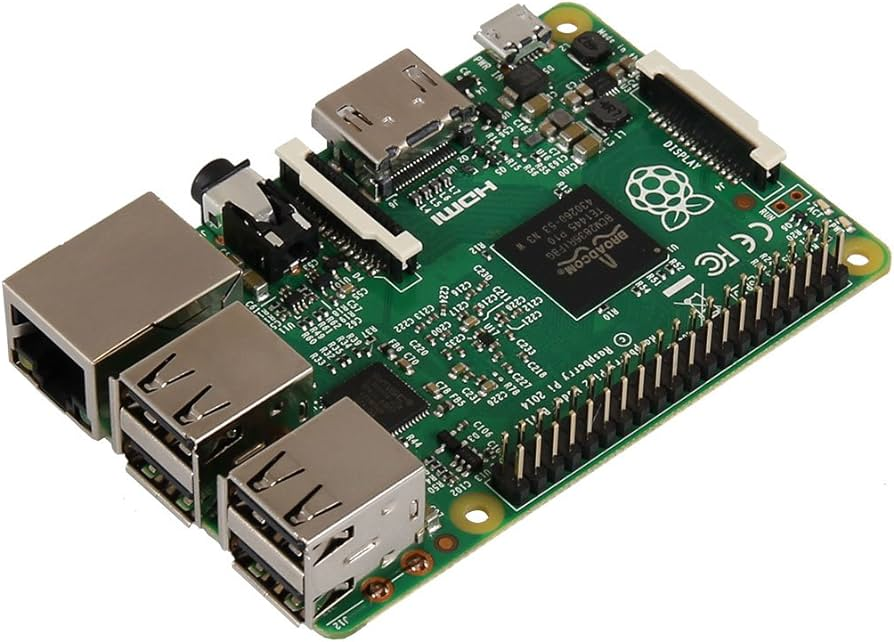
\includegraphics[width=0.5\textwidth]{images/raspimg.jpg}
\caption{Raspberry Pi 4 Model B}

\end{figure}

\section{Software Overview}

\subsection{ESRGAN for Image Super-Resolution}
\begin{figure}[H]
    \centering
    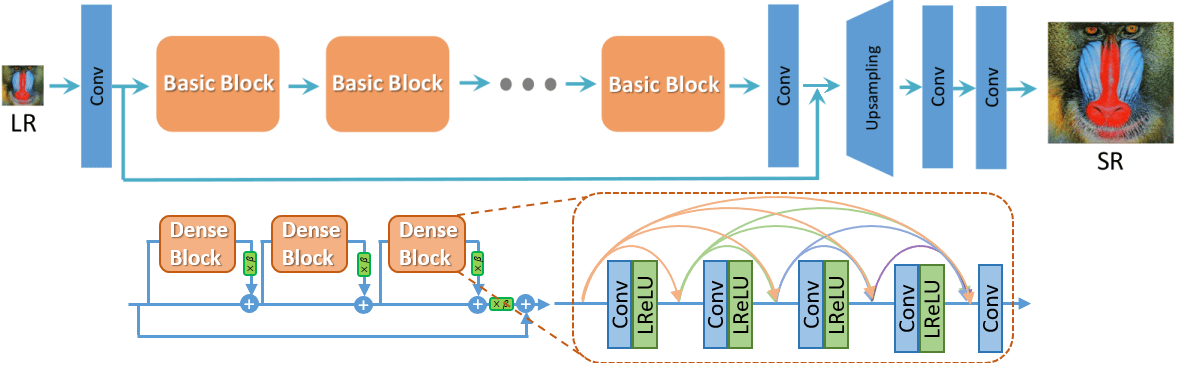
\includegraphics[width=0.85\linewidth]{images/esrganarchi.png}
    \caption{ESRGAN Architecture with Residual-in-Residual Dense Blocks (RRDB)}
    \label{fig:esrgan}
\end{figure}
ESRGAN introduced by Wang \emph{et al.} in 2018 [1], improves upon SRGAN by employing a deep generator built from Residual‑in‑Residual Dense Blocks (RRDB) without batch normalization. Each RRDB combines multiple convolutional layers, local dense connections, and global residual links to capture complex image features. The generator upsamples low‑resolution inputs (e.g.\ 820×616 pixels) by a factor of 4× to high‑resolution outputs (e.g.\ 3280×2464 pixels). The discriminator is relativistic, estimating the probability that a real image is more realistic than a generated one, which enhances stability and visual fidelity. ESRGAN further integrates a perceptual loss based on high‑level VGG features computed before ReLU activations, preserving fine textures and brightness consistency. This design enables ESRGAN to produce photorealistic details, as demonstrated by its victory in the PIRM2018 SR Challenge [1].

In our UAV system, images captured onboard with a Raspberry Pi USB Camera are retrieved post‑flight. ESRGAN runs on a ground PC to upscale extracted frames, recovering critical details (e.g.\ building outlines, vegetation patterns) necessary for accurate land use classification in the Kathmandu region.

\subsection{Comparison of Super-Resolution Models}
We compare ESRGAN with earlier SR approaches:

\begin{table}[H]
\centering
\renewcommand{\arraystretch}{1.2}
\setlength{\tabcolsep}{6pt}
\begin{tabular}{@{} l l p{3cm} p{3cm} p{3cm} @{}}
    \toprule
    \textbf{Model} & \textbf{Year} & \textbf{Architecture} & \textbf{Strengths} & \textbf{Weaknesses} \\
    \midrule
    SRCNN   & 2014 & 3-layer CNN & Simple, fast & Overly smooth outputs [2] \\
    FSRCNN  & 2016 & CNN + deconv & Efficient, higher PSNR [2] & Limited texture detail \\
    EDSR    & 2017 & Deep ResNet & High PSNR, faster [3] & Less perceptual quality \\
    ESRGAN  & 2018 & GAN + RRDB & Realistic textures, sharp edges [1] & Computationally intensive \\
    \bottomrule
  \end{tabular}
  \caption{Comparison of Super-Resolution Models}
\label{tab:sr_models}
\end{table}


\subsection{Land Use Classification}
Land use classification from UAV imagery entails categorizing pixels or patches into classes such as forest, agriculture, water, and urban. Common approaches include:
\begin{itemize}
  \item \textbf{Convolutional Neural Networks (CNNs)}: End‑to‑end models (e.g.\ U‑Net, ResNet, EfficientNet) that learn spatial hierarchies directly from upscaled images [4].
  \item \textbf{Random Forest (RF)}: Ensemble of decision trees trained on raw pixels or derived indices, robust to overfitting and effective for moderate datasets [2,4].
  \item \textbf{Support Vector Machine (SVM)}: Kernel‑based classifier suitable for moderate‑sized, well‑separated classes [2,4].
\end{itemize}
A hybrid approach often combines CNN feature extractors with RF or SVM classifiers, leveraging deep networks for hierarchical feature learning and traditional ML for robust classification when labeled data is limited.

\subsection{Software}
The software pipeline integrates the following tools and libraries:
\begin{itemize}
  \item \textbf{OpenCV}: For image/frame extraction, filtering, and geometric transformations [5].
  \item \textbf{NumPy \& SciPy}: Core numerical and array operations for preprocessing.
  \item \textbf{scikit-learn}: Implements RF and SVM classifiers, data splitting, scaling, and evaluation utilities [6].
  \item \textbf{TensorFlow \& PyTorch}: Deep learning frameworks for ESRGAN and CNN implementation. PyTorch (BasicSR toolkit) eases experimentation [7], while TensorFlow (TF‑Hub ESRGAN) supports scalable deployment [8].
  \item \textbf{GDAL/Rasterio}: For handling geo-referenced imagery and aligning with regional GIS data [9].
\end{itemize} 


\subsection{Dataset}

\textbf{1. Kathmandu Land Use Datasets}

Region-specific datasets used for land use classification in Kathmandu:

\begin{itemize}
  \item \textbf{Nepal National Land Cover Dataset}: Annual land-cover maps (2000–2022) from Landsat imagery via Google Earth Engine, covering forests, agriculture, water, and built-up areas[10].
  \item \textbf{Kathmandu City Land Use Shapefiles}: Urban land use polygons (residential, commercial, parks) for Kathmandu Metropolitan City (2011) from ICIMOD[11].
  \item \textbf{OpenStreetMap Polygons}: Land-use tags for Kathmandu accessible through the Humanitarian Data Exchange[12].
\end{itemize}

\textbf{2. Image Super-Resolution Datasets}

Datasets used to train and evaluate ESRGAN and other super-resolution models:

\begin{itemize}
  \item \textbf{DIV2K}: A large-scale dataset designed for image super-resolution, consisting of 1000 high-resolution images and their corresponding low-resolution counterparts. Suitable for training deep SR models.
  \item \textbf{Set5 and Set14}: Benchmark datasets commonly used for evaluating the performance of super-resolution models. While smaller in size, they are widely adopted for quantitative comparisons.
\end{itemize}

These datasets provide essential ground truth for training and validating both our land use classification pipeline and image super-resolution models.



\chapter{Feasibility Study}
\label{feasiblity}
\section{Technical Feasibility}
\begin{table}[h]
\caption{Hardware Specification Table}
\vspace{12pt}
\centering
\begin{tabular}{|c|c|c|}
\hline
Column 1 & Column 2 & Column 3 \\
\hline
Item 1   & Item 2   & Item 3   \\
Item 4   & Item 5   & Item 6   \\
Item 7   & Item 8   & Item 9   \\
\hline
\end{tabular}

\label{tab:Hardware Specification Table}
\end{table}
\section{Economic Feasibility}
\lipsum[4-8]



\chapter{Methodology}
\label{methodology}
\section{System Block Diagram}
\lipsum[4-8]
\section{Flow Chart}
\lipsum[4-8]

\chapter{Expected Output}
\label{result}
\section{Expected Output}

 The project aims to develop an innovative interactive gesture-controlled gaming system that
 translates real-hand movements into precise in-game character actions. The primary output will
 be a custom-designed wearable interface integrating MPU sensors, and mechanical switches
 enabling accurate hand gesture detection. The system will facilitate real-time data transmission
 between hardware and gameengine, creating an immersive first-person gaming experience with
 minimal latency. Key deliverables include a responsive input mechanism, gesture recognition
 algorithm, and puzzle game prototype demonstrating seamless hardware-software interaction.
 The project seeks to achieve 90 percent gesture detection accuracy, showcasing potential ad
vancements in interactive gaming technologies through innovative human-computer interface
 design.
 

\chapter*{Gantt Chart}
\addcontentsline{toc}{chapter}{Gantt Chart}
\label{ganttchart}
\begin{figure}[ht]
    \centering
    
\includegraphics[scale=0.45]{images/kec.png}
\end{figure}

\chapter*{Cost Estimation}
\addcontentsline{toc}{chapter}{Cost Estimation}
\label{cost estimation}
 
% Table 1: Electronics & Core Components
\section*{Electronics \& Core Components}
\begin{table}[h]
\centering
\begin{tabular}{l c S[table-format=5.0]}
\toprule
\textbf{Item} & \textbf{Quantity} & \textbf{Cost (NRs)} \\
\midrule
FLYSKY Receiver & 1 & 8000 \\
30A ESC Skywalker & 1 & 2000 \\
Flight Stabilizer (NXE4 EVO) & 1 & 4500 \\
1000KV Brushless Motor & 1 & 800 \\
MG996 Metal Gear Servo & 4 & 3040 \\
2200mAh 3S LiPo Battery & 1 & 3150 \\
Buck Module Voltage Regulator & 1 & 550 \\
Raspberry Pi 4B with USB Camera and HDMI Cable & 1 & 0 \\
\midrule
\textbf{Total} & & \textbf{22040} \\
\bottomrule
\end{tabular}
\caption{Electronics and Core Components for Fixed-Wing UAV}
\end{table}

\section*{Frame \& Construction Materials}
\begin{table}[h]
\centering
\begin{tabular}{l c S[table-format=5.0]}
\toprule
\textbf{Item} & \textbf{Quantity} & \textbf{Cost (NRs)} \\
\midrule
Depron Sheet(1000*600 mm) & 4 & 10000 \\
Aluminum Motor Mount (L-shape) & 1 & 150 \\
Push Rod (1m) & 2 & 400 \\
\midrule
\textbf{Total} & & \textbf{10550} \\
\bottomrule
\end{tabular}
\caption{Frame and Construction Materials for Fixed-Wing UAV}
\end{table}

\newpage
\section*{Miscellaneous Accessories}
\begin{table}[h]
\centering
\begin{tabular}{l c S[table-format=4.0]}
\toprule
\textbf{Item} & \textbf{Quantity} & \textbf{Cost (NRs)} \\
\midrule
Hot Glue Gun Stick & 10 & 200 \\
Duct/Binding Tape & 3 rolls & 300 \\
XT60 Connector Pair & 2 & 500 \\
3-Pin Orange Connector Pair & 4 & 60 \\
Servo Wire Cable (5m) & 1 & 75 \\
Propeller (7x5 inch) & 4 & 300 \\
Bullet Propeller Holder Adapter & 1 & 170 \\
Jumper Wire (MM, MF, FF, each 5) & 15 & 30 \\
\midrule
\textbf{Total} & & \textbf{1635} \\
\bottomrule
\end{tabular}
\caption{Miscellaneous Accessories for Fixed-Wing UAV}
\end{table}

\section*{Grand Total}
\begin{table}[h]
\centering
\begin{tabular}{l S[table-format=5.0]}
\toprule
\textbf{Category} & \textbf{Cost (NRs)} \\
\midrule
Electronics and Core Components & 22040 \\
Frame and Construction Materials & 10550 \\
Miscellaneous Accessories & 1635 \\
\midrule
\textbf{Grand Total} & \textbf{34225} \\
\bottomrule
\end{tabular}
\caption{Grand Total Cost for Fixed-Wing UAV}
\end{table}



\chapter*{References}
\addcontentsline{toc}{chapter}{References}
\label{references}
\begin{enumerate}
  \item X. Zhang, M. Liu, and Y. Zhao, “Design of angle detection system based on MPU6050,” in \textit{Proc. Int. Conf. Intelligent Transportation, Big Data \& Smart City}, Changsha, China, 2017, pp. 159–162.
  \item S. J. Park and S. Y. Lee, “Real-Time Motion Recognition Using an Accelerometer,” \textit{Sensors}, vol. 15, no. 1, pp. 135–148, 2015.
  \item P. Kumar, J. Verma, and S. Prasad, “Hand Data Glove: A Wearable Real-Time Device for Human-Computer Interaction,” \textit{Int. J. Adv. Sci. Technol.}, vol. 43, pp. 15–23, Jun. 2012.
  \item A. Khandual and A. Biswal, “IoT Based Smart Glove for Hand Gesture Recognition,” \textit{Int. J. Sci. Res. Comput. Sci. Eng. Inf. Technol.}, vol. 5, no. 2, pp. 384–389, Mar. 2019.
  \item M. Nasri et al., “Design and Implementation of a 3D Printed Hand Gesture Recognition System Using Arduino and Flex Sensors,” \textit{IEEE Access}, vol. 7, pp. 55371–55378, 2019.
  \item T. Baudel and M. Beaudouin-Lafon, “Charade: Remote Control of Objects Using Free-Hand Gestures,” \textit{Commun. ACM}, vol. 36, no. 7, pp. 28–35, 1993.
  \item Rautaray, S. S., \& Agrawal, A. (2013). Real-time hand gesture recognition system       for dynamic applications. International Journal of UbiComp, 4(3), 21–35.
  \item Chowdhury, S., \& Haque, A. (2013). Animatronic hand controller. 
  \item Kumar, P., Verma, J., \& Prasad, S. (2012). Hand data glove: A wearable real-time device for human-computer
  \item Sturman, D. J., \& Zeltzer, D. (1994). A survey of glove-based input. *IEEE Computer Graphics and Applications, 14*(1), 30-39.
  \item Huang, J. (2017). Design of angle detection system based on MPU6050. *Advances in Computer Science Research, 73*, 1-3.
\end{enumerate}
%\bibliographystyle{plain} % or another style like ieee, unsrt, etc.
%\bibliography{references} % references.bib (no .bib extension)


\end{document}
